\documentclass[border=6pt]{standalone}
\usepackage{tikz}
\usetikzlibrary{arrows.meta,positioning,fit,backgrounds,calc}
\usepackage[T1]{fontenc}
\usepackage{lmodern}
\begin{document}
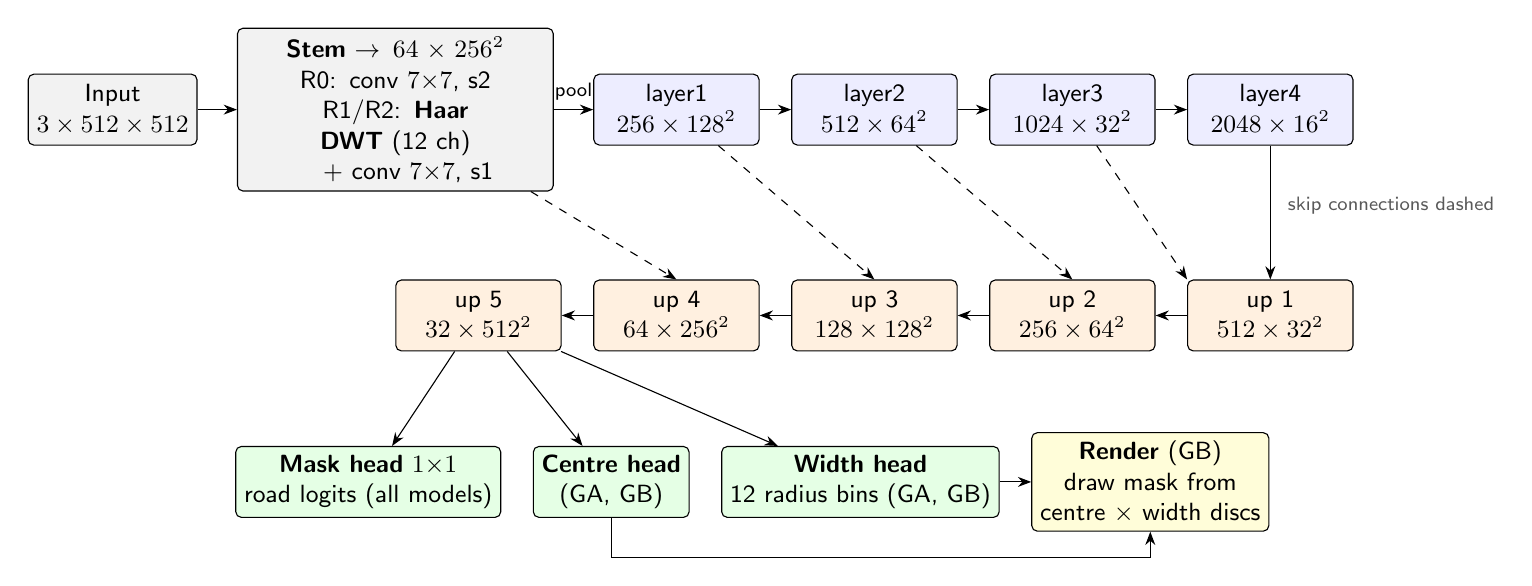
\begin{tikzpicture}[
  font=\sffamily\small, >=Stealth,
  box/.style={draw, rounded corners=2pt, align=center, inner sep=3pt, minimum height=9mm},
  enc/.style={box, fill=blue!7, minimum width=21mm}, dec/.style={box, fill=orange!12, minimum width=21mm},
  op/.style={box, fill=gray!10}, head/.style={box, fill=green!10}, var/.style={box, fill=red!6, text width=50mm, align=left}]

\node[op] (in) {Input\\$3\times512\times512$};
\node[op, right=5mm of in, text width=38mm] (stem) {\textbf{Stem} $\to 64\times256^2$\\R0: conv $7{\times}7$, s2\\R1/R2: \textbf{Haar DWT} (12 ch)\\\quad + conv $7{\times}7$, s1};
\node[enc, right=5mm of stem] (l1) {layer1\\$256\times128^2$};
\node[enc, right=4mm of l1] (l2) {layer2\\$512\times64^2$};
\node[enc, right=4mm of l2] (l3) {layer3\\$1024\times32^2$};
\node[enc, right=4mm of l3] (l4) {layer4\\$2048\times16^2$};
\draw[->] (in) -- (stem); \draw[->] (stem) -- node[above, font=\sffamily\scriptsize]{pool} (l1);
\draw[->] (l1) -- (l2); \draw[->] (l2) -- (l3); \draw[->] (l3) -- (l4);

\node[dec, below=17mm of l4] (d1) {up 1\\$512\times32^2$};
\node[dec, left=4mm of d1] (d2) {up 2\\$256\times64^2$};
\node[dec, left=4mm of d2] (d3) {up 3\\$128\times128^2$};
\node[dec, left=4mm of d3] (d4) {up 4\\$64\times256^2$};
\node[dec, left=4mm of d4] (d5) {up 5\\$32\times512^2$};
\draw[->] (l4) -- (d1); \draw[->] (d1) -- (d2); \draw[->] (d2) -- (d3); \draw[->] (d3) -- (d4); \draw[->] (d4) -- (d5);
\draw[->, dashed] (l3) -- (d1.north west);
\draw[->, dashed] (l2) -- (d2.north); \draw[->, dashed] (l1) -- (d3.north); \draw[->, dashed] (stem) -- (d4.north);
\node[font=\sffamily\scriptsize, gray!70!black, anchor=west] at ($(l4.south)!0.45!(d1.north)+(1mm,0)$) {skip connections dashed};

\node[head, below=12mm of d5, xshift=-14mm] (mh) {\textbf{Mask head} $1{\times}1$\\road logits (all models)};
\node[head, right=4mm of mh] (ch) {\textbf{Centre head}\\(GA, GB)};
\node[head, right=4mm of ch] (wh) {\textbf{Width head}\\12 radius bins (GA, GB)};
\node[head, right=4mm of wh, fill=yellow!15] (rd) {\textbf{Render} (GB)\\draw mask from\\centre $\times$ width discs};
\draw[->] (d5) -- (mh); \draw[->] (d5) -- (ch); \draw[->] (d5) -- (wh);
\draw[->] (wh) -- (rd); \draw[->] (ch.south) -- ++(0,-5mm) -| (rd.south);

\end{tikzpicture}
\end{document}
